\section{Systematic uncertainties}
\label{sec:syst}
We consider several sources of systematic uncertainty, taking into
account their effect on both the signal acceptance and on the template
shapes for the signal extraction fit.  The uncertainty on the
normalization of the backgrounds is taken as part of the statistical
uncertainty.  The largest source of systematic uncertainty is the
shape uncertainty of the W+jets template.  Other sources of systematic
uncertainty considered include jet energy scale (JES) as well as
trigger and lepton identification efficiencies.
%%%%%%%%%%%%%%%%%%%%%%%%%%%%%%%%%%%%%%%%%%%%
\subsection{Systematics due to the W+jets shape}
\label{sec:syst_mjj}
%%%%%%%%%%%%%%%%%%%%%%%%%%%%%%%%%%%%%%%%%%%%%
The $m_{jj}$ shape for W+jets events is taken from the MC.  Its shape
could be different due to NLO corrections and other effects.
Figure~\ref{fig:wjetshapes} shows possible shapes derived from our MC
samples.  To evaluate the effect of these shapes and propagate them
into our limit, we use the five MadGraph samples, which are the large
statistics nominal sample, one sample with the $q^2$ factorization and
renormalization scale doubled, one with the $q^2$ scale halved, one
with the matching scale doubled and one with the matching scale
halved.  We find an ``optimal'' mixture of the MC samples during our
nominal fit and its uncertainty is propagated by the fitter into the
yields and thus into our final limit. %the technique described in
%Section~\ref{sec:wjetsShape} separately for the 2- and 3-jet bins.
%The shapes that are produced corresponding to the different systematic
%variations on the parameters are propagated to the limit setting as a
%systematic error.

%\subsubsection{Uncertainty due to limited amount of MC}
%The main source of systematic error on the W+jets shape is due to the limited amount of MC
%events in the samples. We evaluate this error by producing Toy MC $m_{jj}$ templates
%based on those from the centrally produced sample. The toy templates are passed through the 
%same optimization procedure and a new optimal mixture is obtained. The resulting uncertainty
%on the W$jj$(Diboson) yield is $XX$($XX$) events for the 2-jet bin and $XX$($XX$) events for 
%the $3$-jet bin.
%Using the distributions of the 
%parameters of the mixture we can evaluate the error on those parameters 
%and propagate that error to the limit setting machinery.

%\subsubsection{Uncertainty due to Factorization Scale and ME-PS Matching}
%The fractions of $q^2$ and matching samples in the overall
%(``optimal'') mixture, obtained from the optimization procedure, have
%corresponding uncertainties.  In order to take the $q^2$-matching
%correlations into account it is necessary to perform a scan in both
%dimensions. Specifically, we vary the scaling and matching fractions
%within $\pm 0.2$ of the optimal values. The systematic error on the
%W$jj$ yield is the difference between the value at the minimum
%-loglikelihood ($nll_{Min}$) and the value at $nll_{Min}+1/2$.
%We scan the $nll_{Min}+1/2$ contour and take the largest difference
%(between the W$jj$ yield at the minimum and on the contour) to be the
%systematic error. The scan results are shown in
%Figs.~\ref{fig:NLL2DScan_2j},~\ref{fig:NLL2DScan_3j}.  The error on
%the W$jj$ yield is 153 events (174 events) in the 2-jet (3-jet) bin.
%%%%%%%%%%%%%%%%%%%%%
%\begin{figure}[htb] 
%  {\centering
%    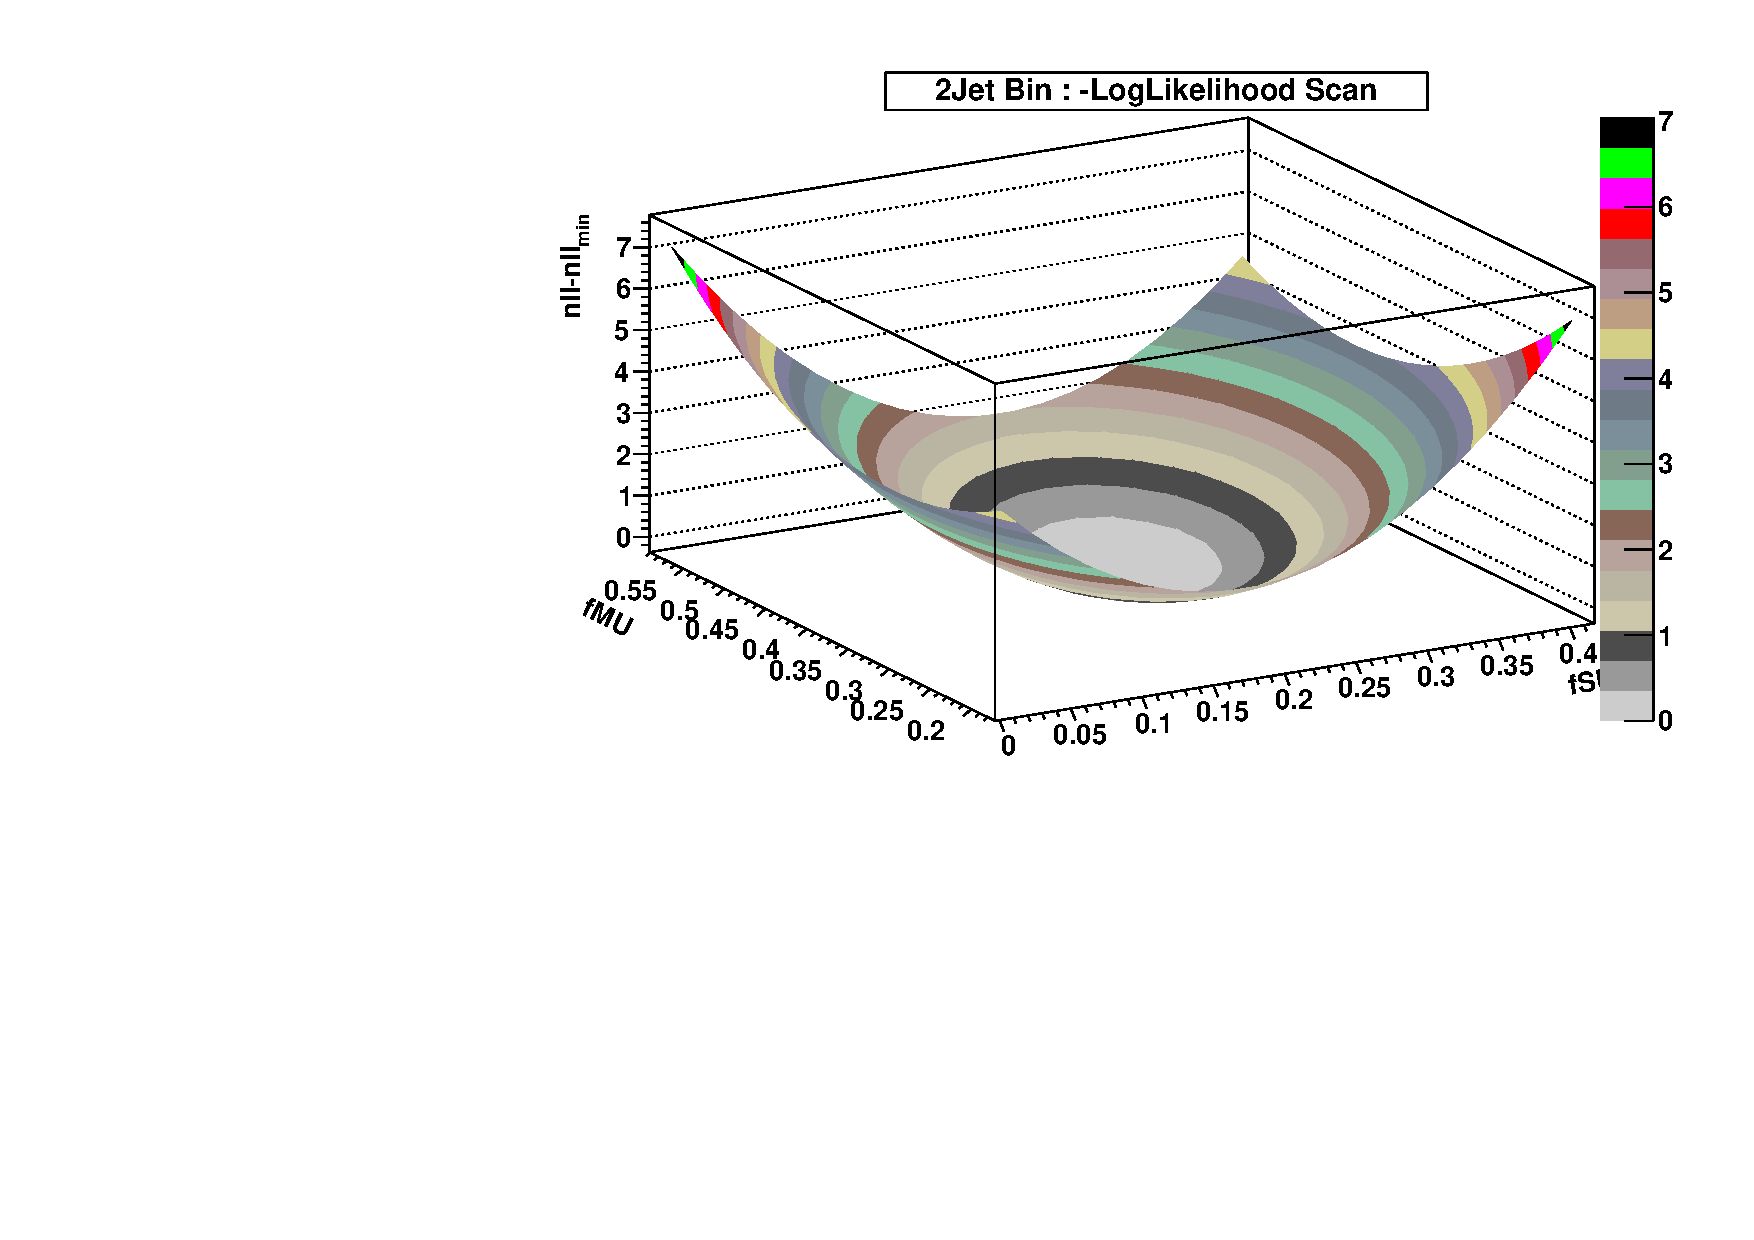
\includegraphics[width=0.49\textwidth]{figs/NLL2DScan_2j_surf.pdf}
%    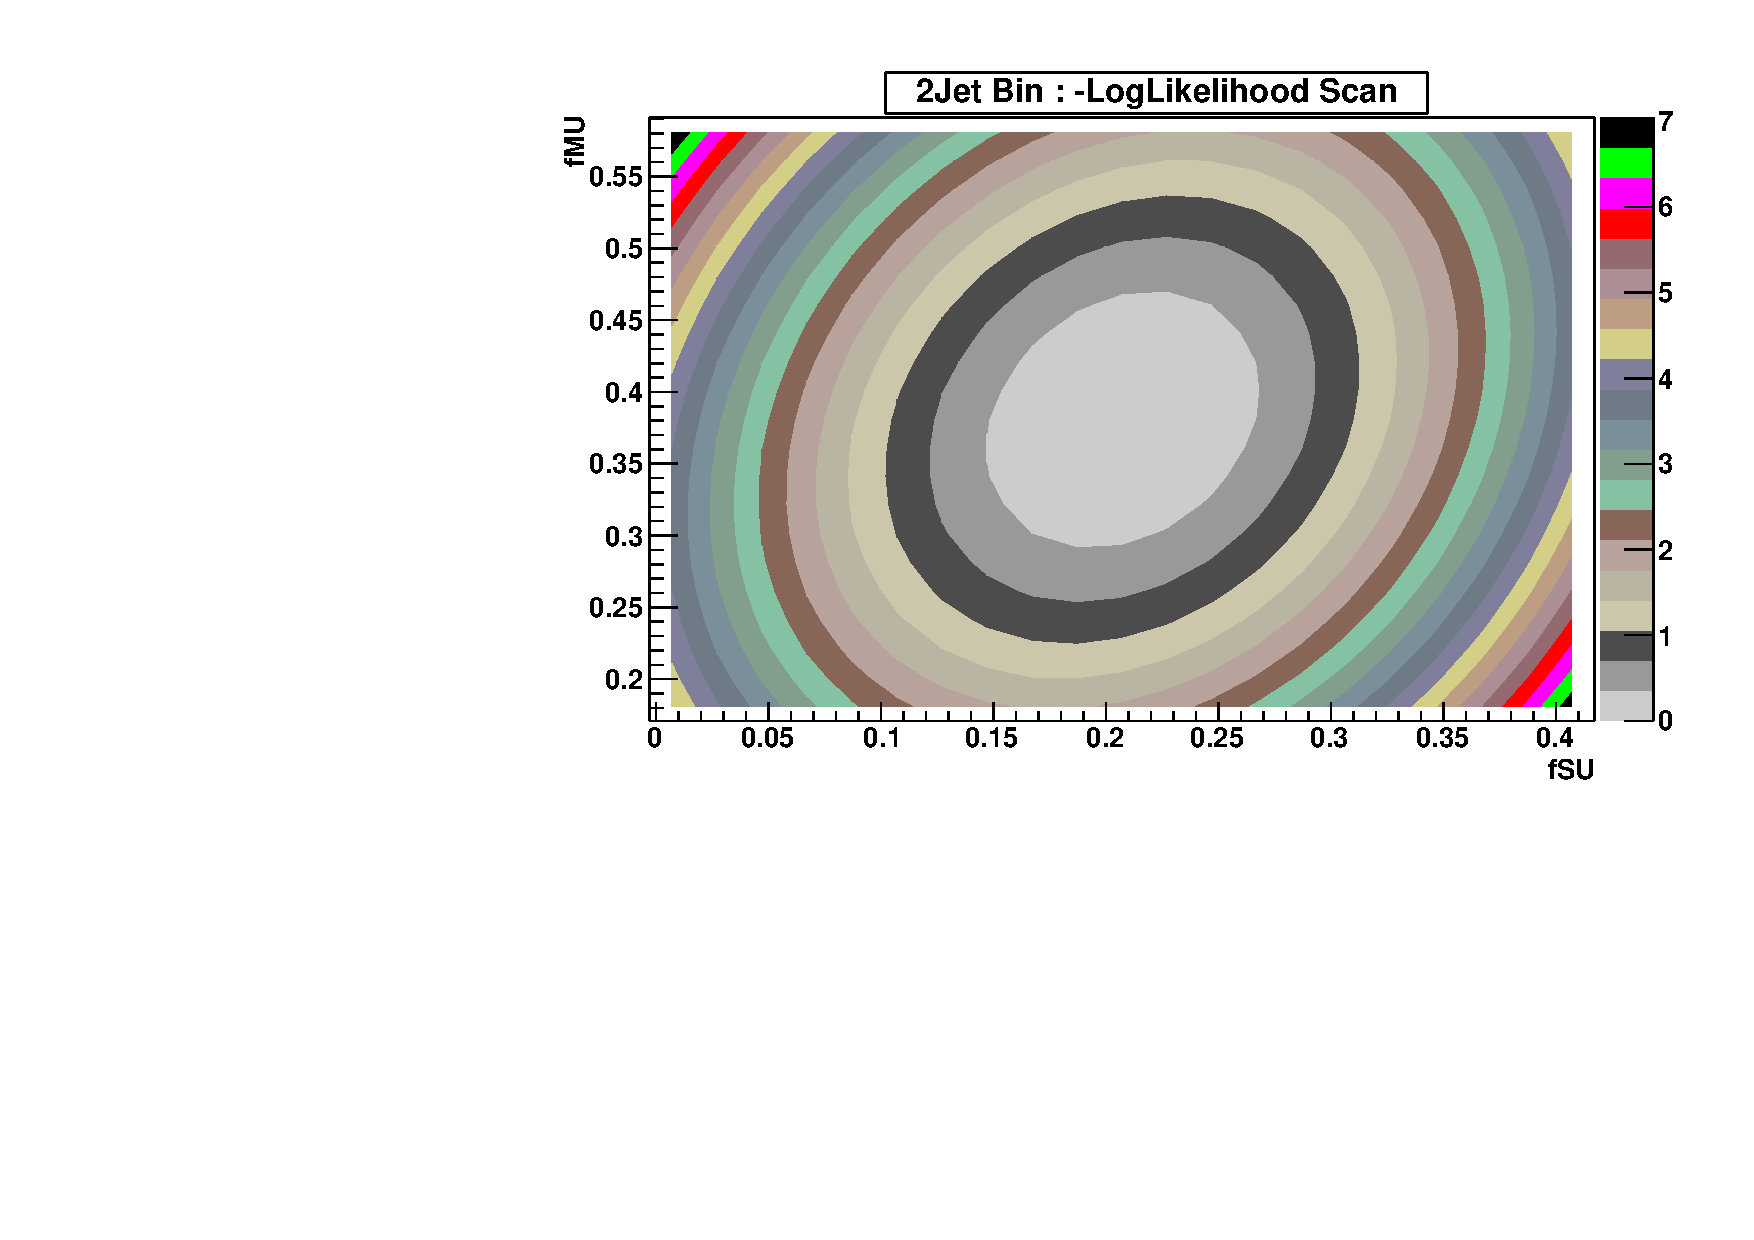
\includegraphics[width=0.49\textwidth]{figs/NLL2DScan_2j_cont.pdf}
%    \caption{Scan over the relative fractions for $q^2$ and matching in the 2-jet bin: Surface (left) and Contour (right).}
%    \label{fig:NLL2DScan_2j}}
%\end{figure}
%%%%%%%%%%%%%%
%\begin{figure}[htb] 
%  {\centering
%    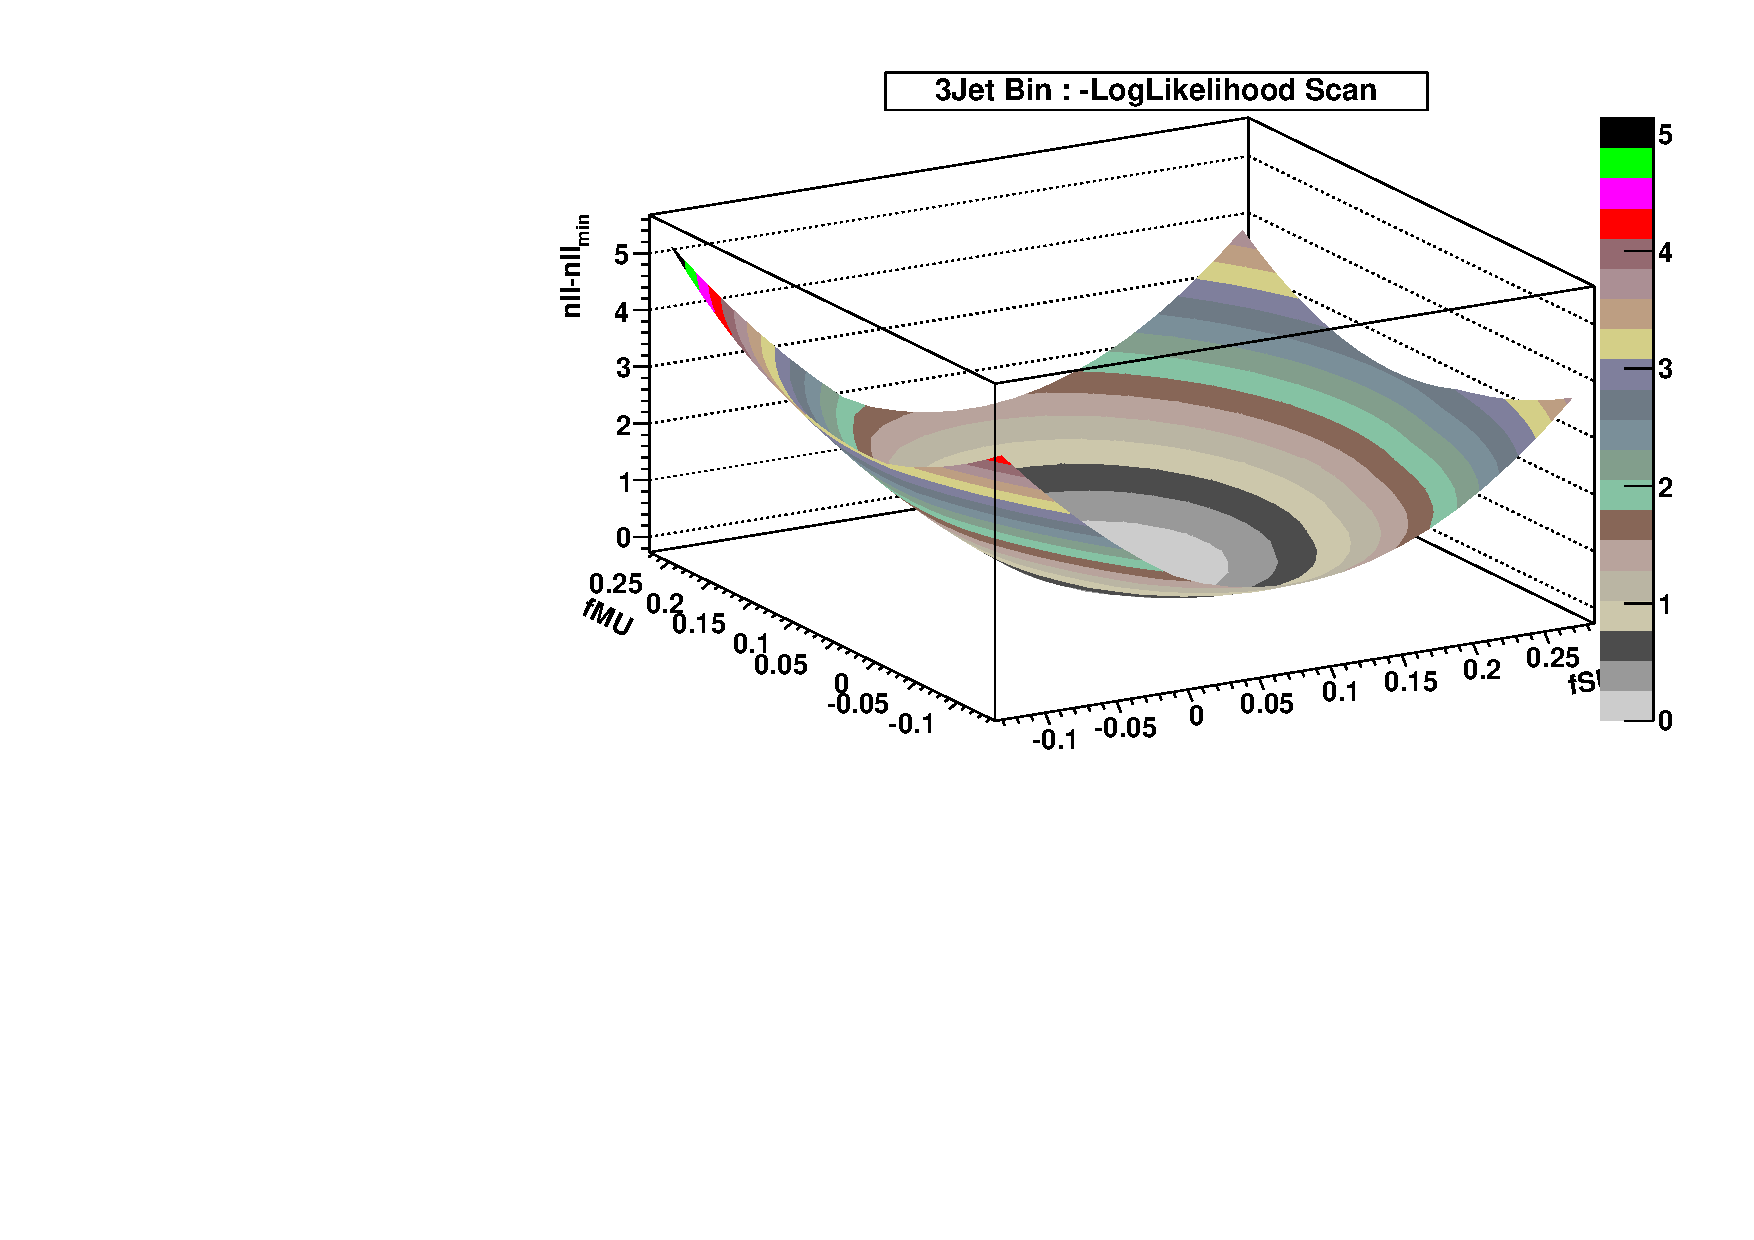
\includegraphics[width=0.49\textwidth]{figs/NLL2DScan_3j_surf.pdf}
%    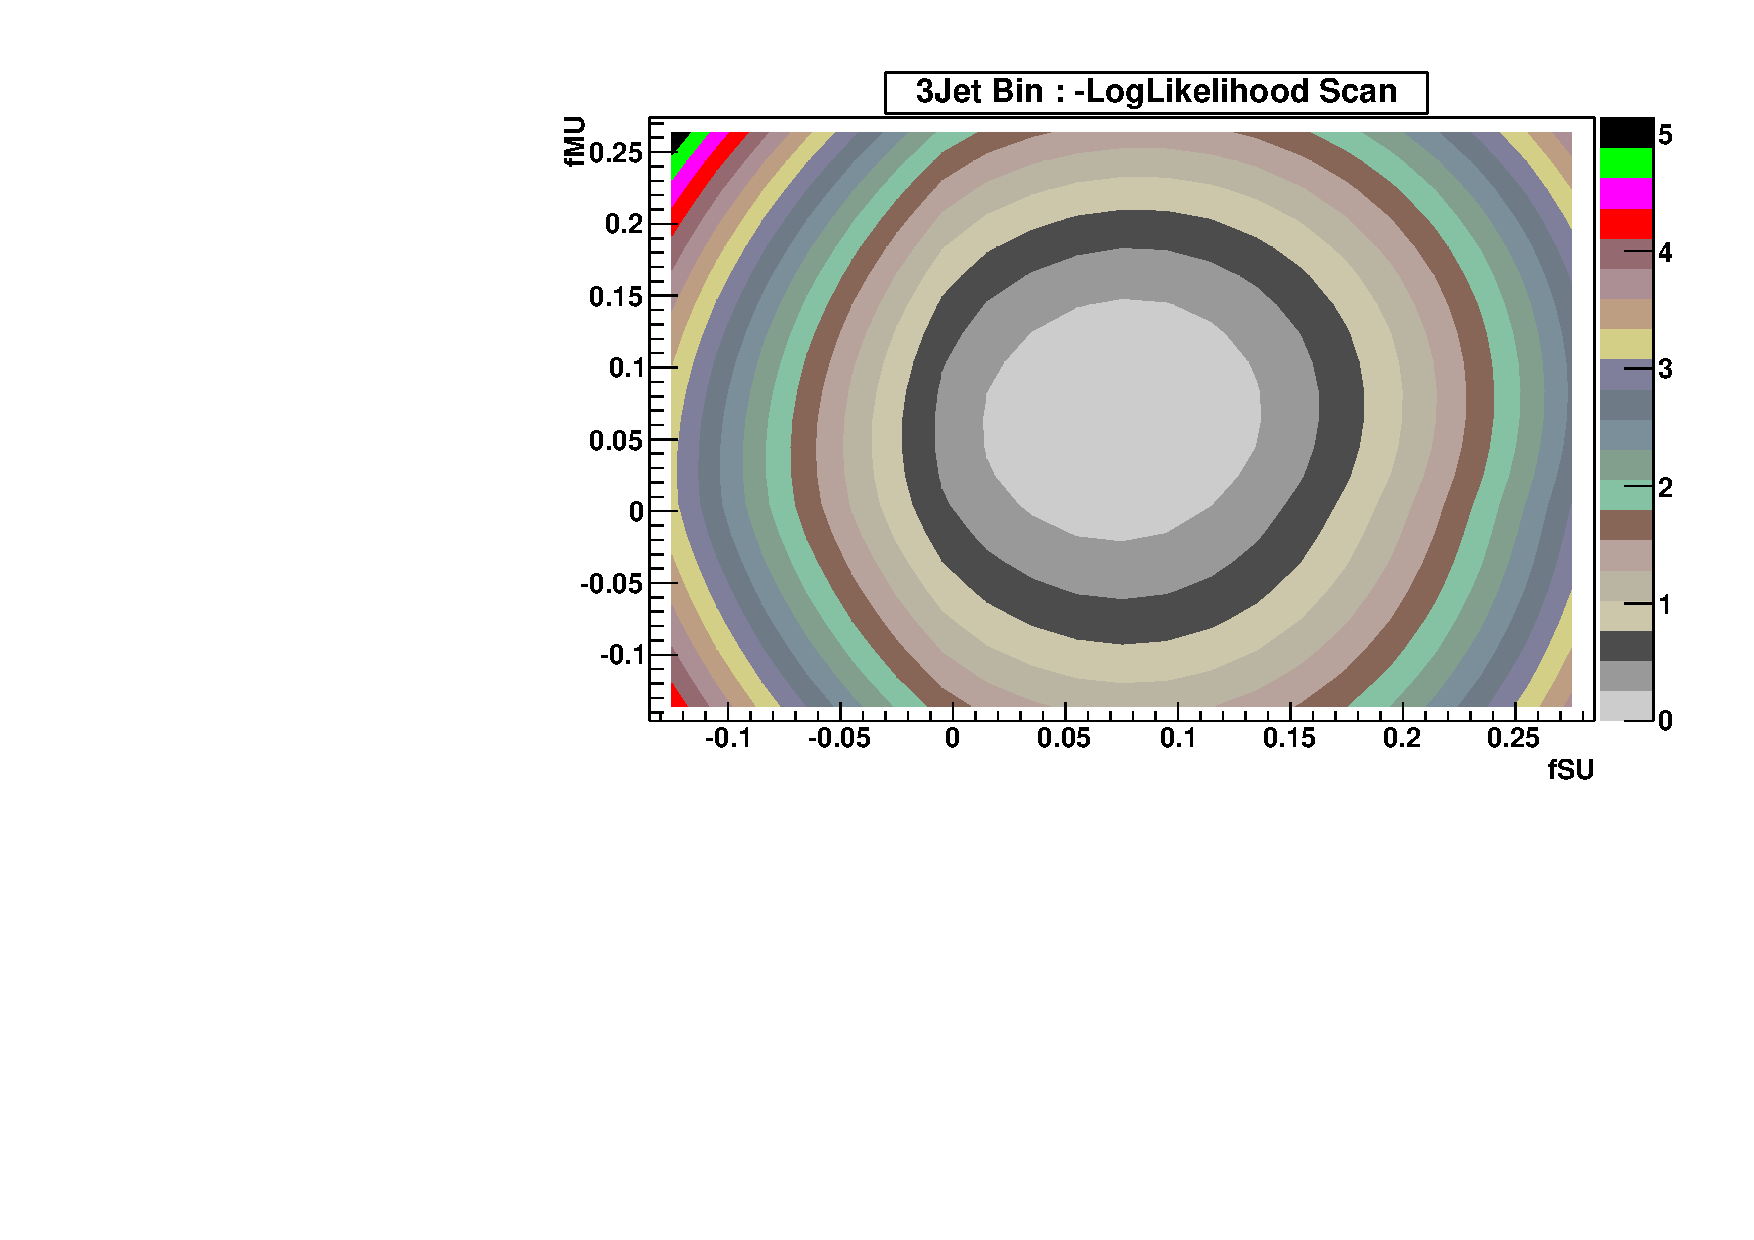
\includegraphics[width=0.49\textwidth]{figs/NLL2DScan_3j_cont.pdf}
%    \caption{Scan over the relative fractions for $q^2$ and matching in the 3-jet bin: Surface (left) and Contour (right).}
%    \label{fig:NLL2DScan_3j}}
%\end{figure}
%%%%%%%%%%%%%%
%%%%%%%%%%%%%%%%%%%%%%%%%%%%%%%%%%%%%%%%
%%%%%%%%%%%%%%%%%%%%%%%%%%%%%%%%%%%%%%%%
\subsection{Jet Energy Scale from the hadronic W in top quark events}
\label{sec:topw}
We reconstruct the hadronic W candidate from an almost pure top data control sample. 
The semileptonic top
events are selected by requiring exactly four jets in the event, out of
which two are b-tagged and the other two are anti-btagged. The
hadronic W candidates are formed from two anti-btagged jets. 
The invariant mass of the hadronic W candidates in the muon,
electron, and combined channels are shown in 
Figs.~\ref{fig:topw:mu},~\ref{fig:topw:el}, and 
\ref{fig:topw:muel}, respectively.  When we propagate the difference in the JES to our
templates they make a negligible difference.
%%%%%%%%%%%%%%%%%%%%%
\begin{figure}[htb] 
  {\centering
    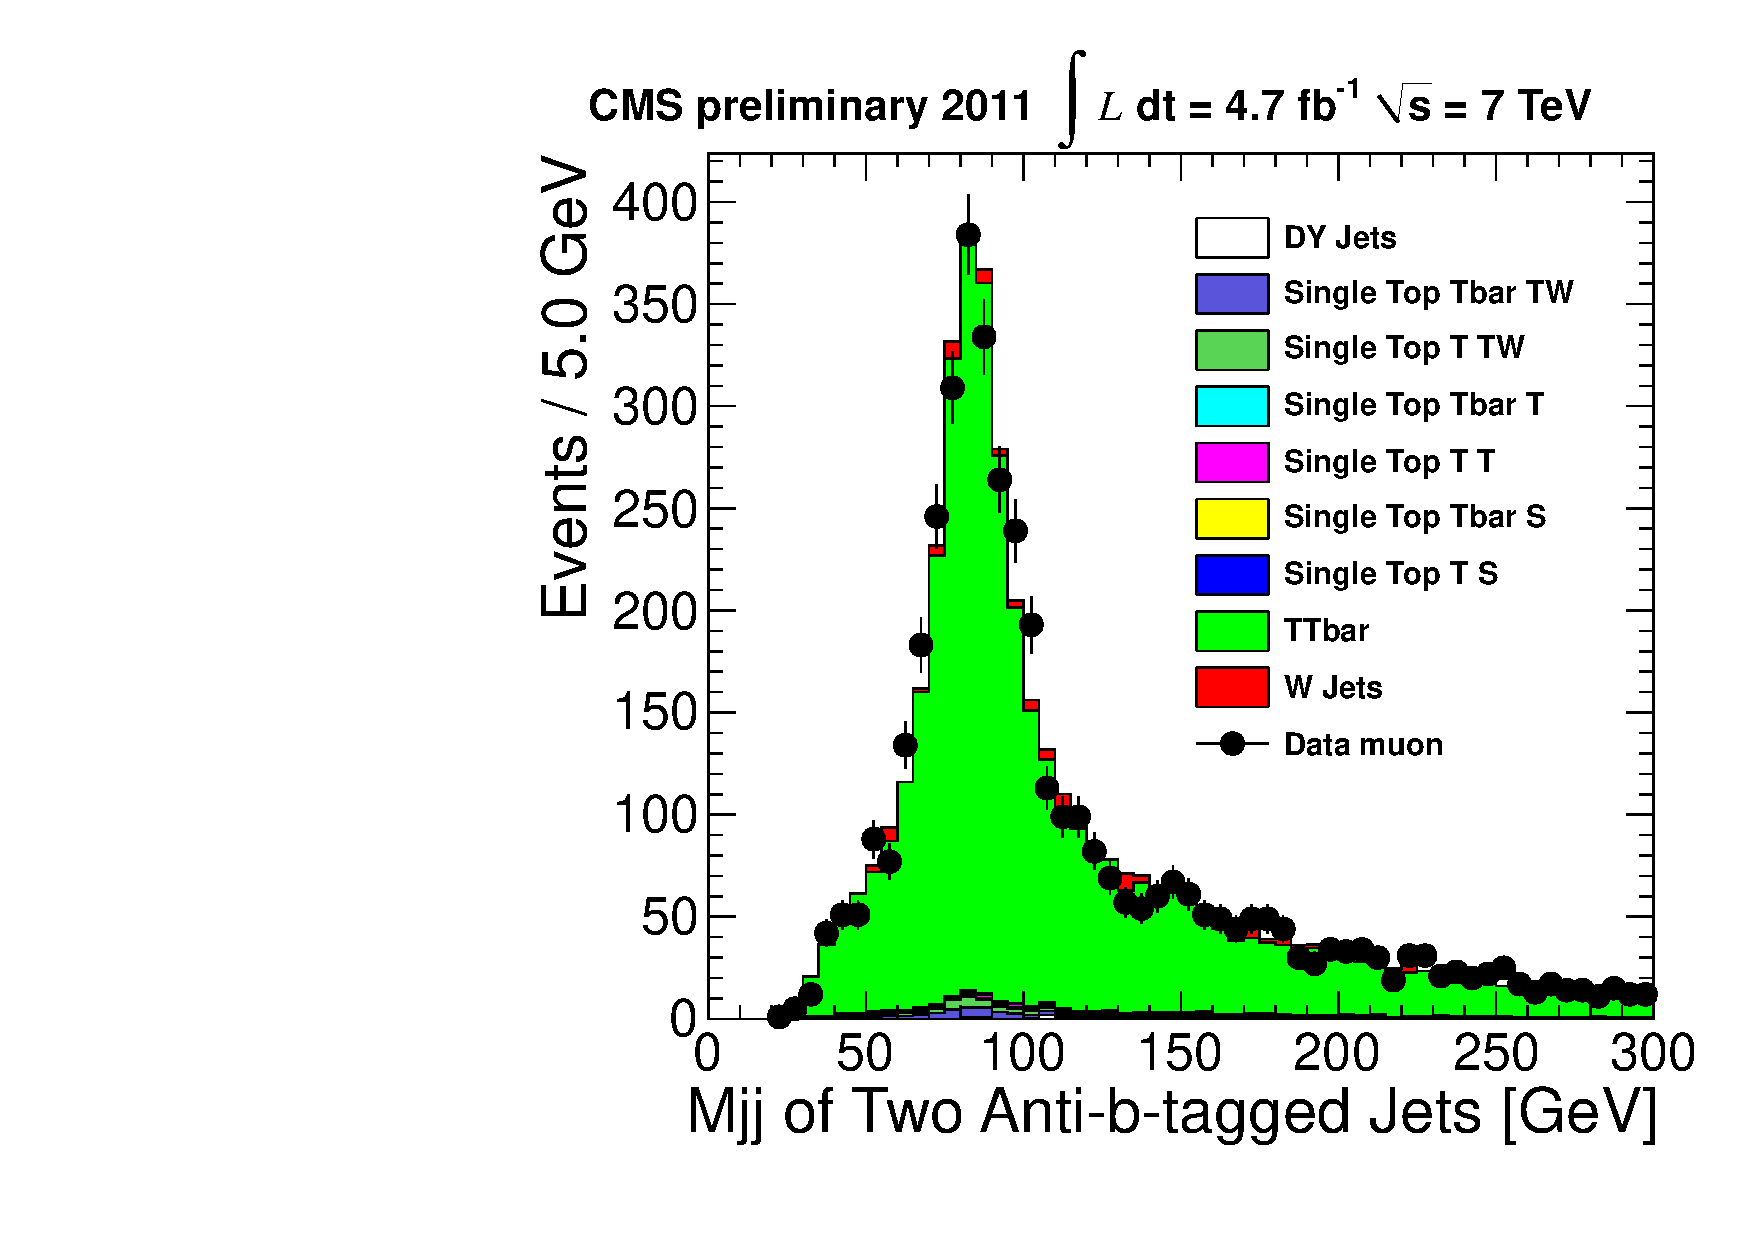
\includegraphics[width=0.75\textwidth]{figs/topwjes/top_overlap_mu.pdf}
    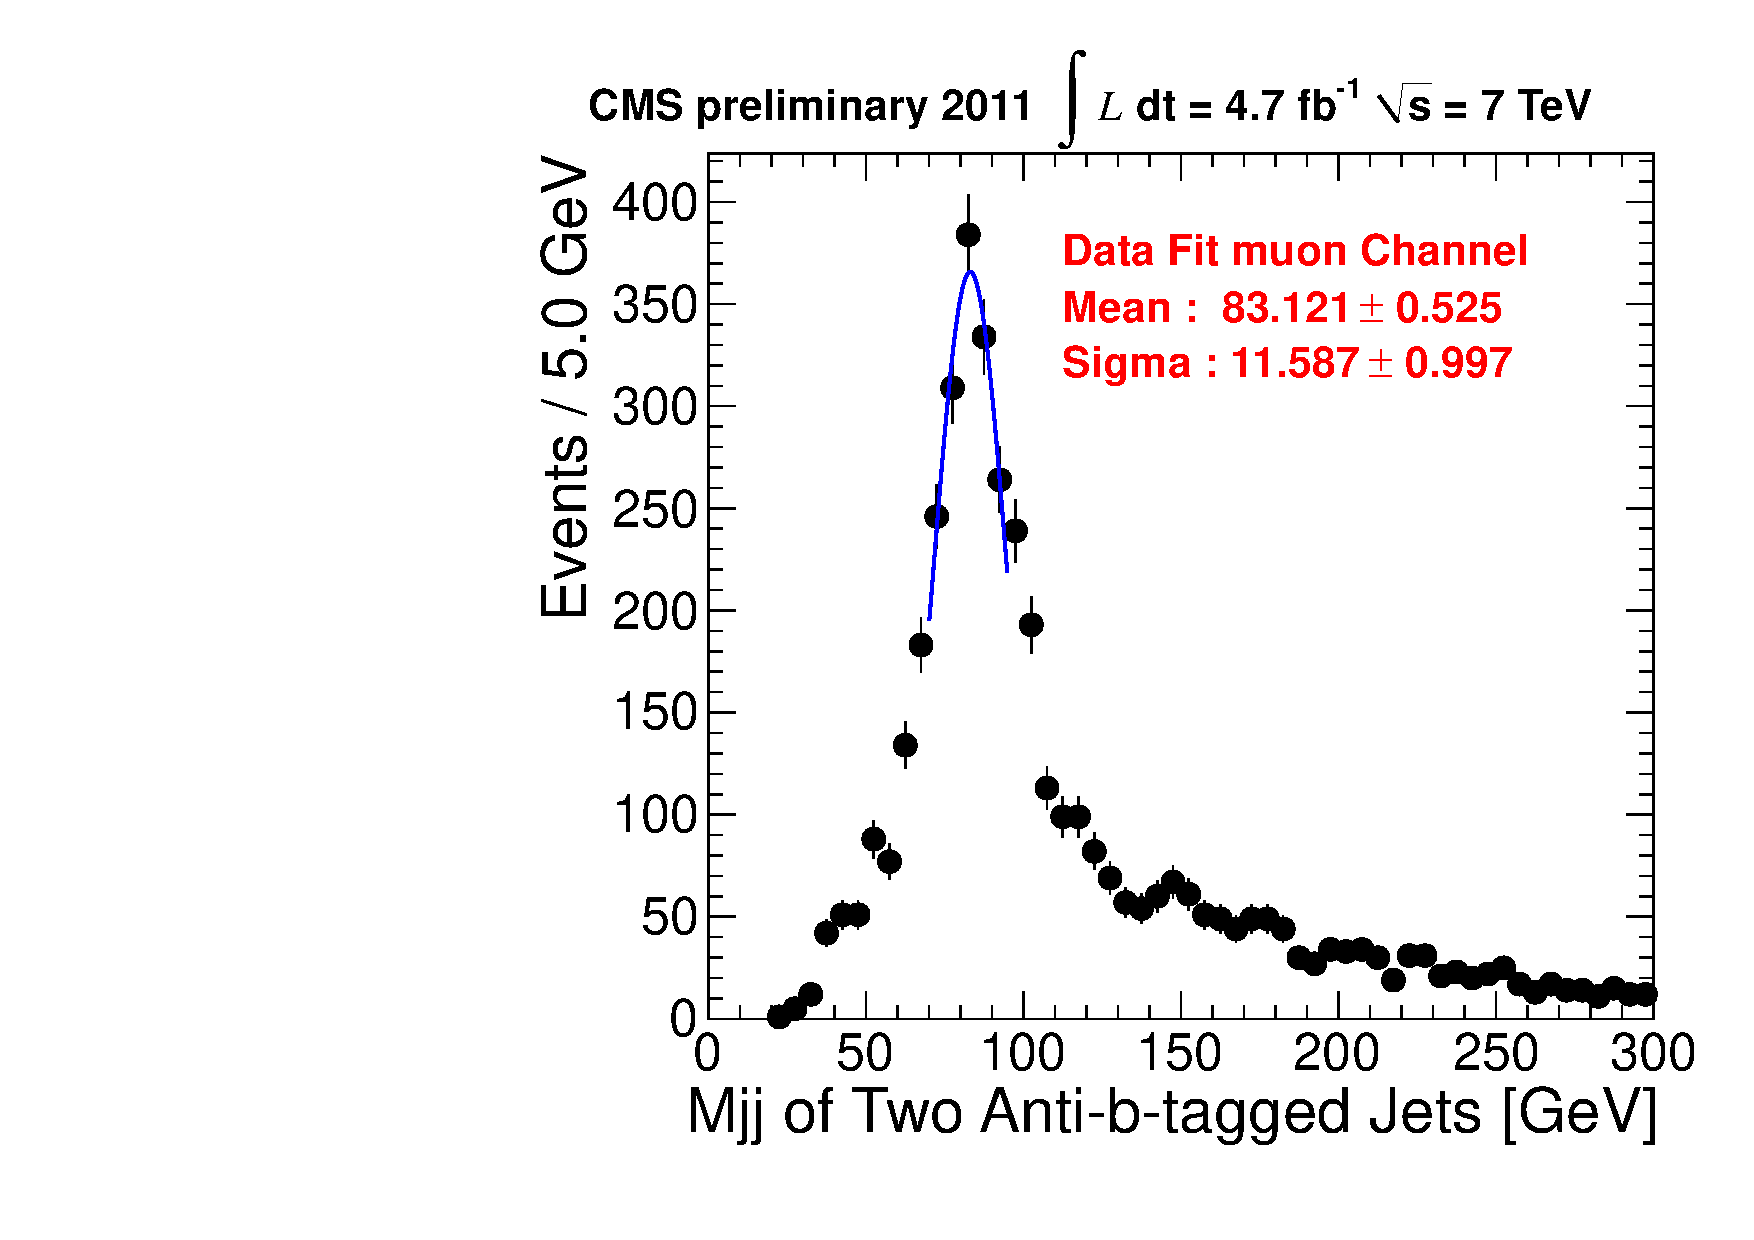
\includegraphics[width=0.49\textwidth]{figs/topwjes/top_data_fit_mu.pdf}
    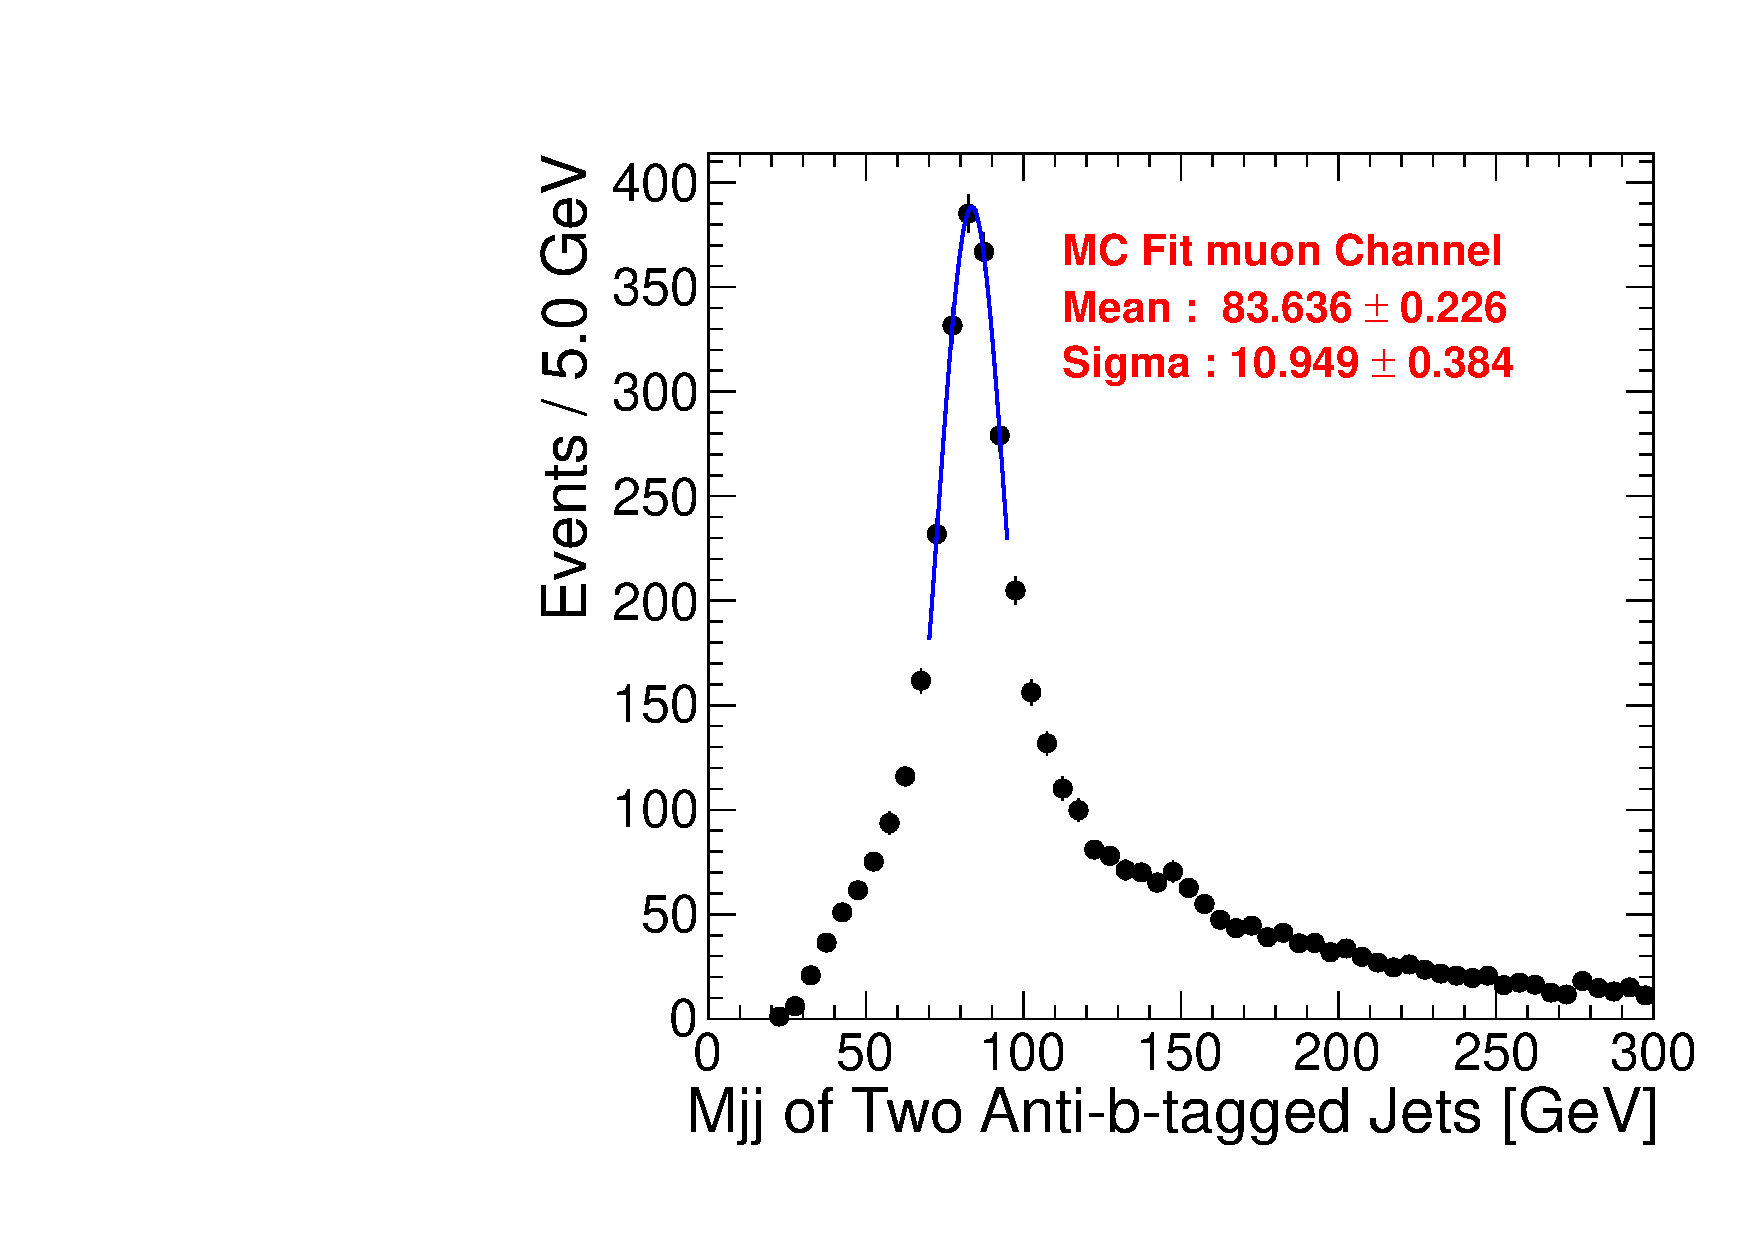
\includegraphics[width=0.49\textwidth]{figs/topwjes/top_mc_fit_mu.pdf}
    \caption{The invariant mass distribution of the hadronic 
      W candidates in the muon semileptonic top sample. 
      The upper plot shows good agreement between the data and MC. 
      We fit the distribution with a Gaussian and extract the peak
      location for the data (left) and MC (right).}
    \label{fig:topw:mu}}
\end{figure}
%%%%%%%%%%%%%%
\begin{figure}[htb] 
  {\centering
    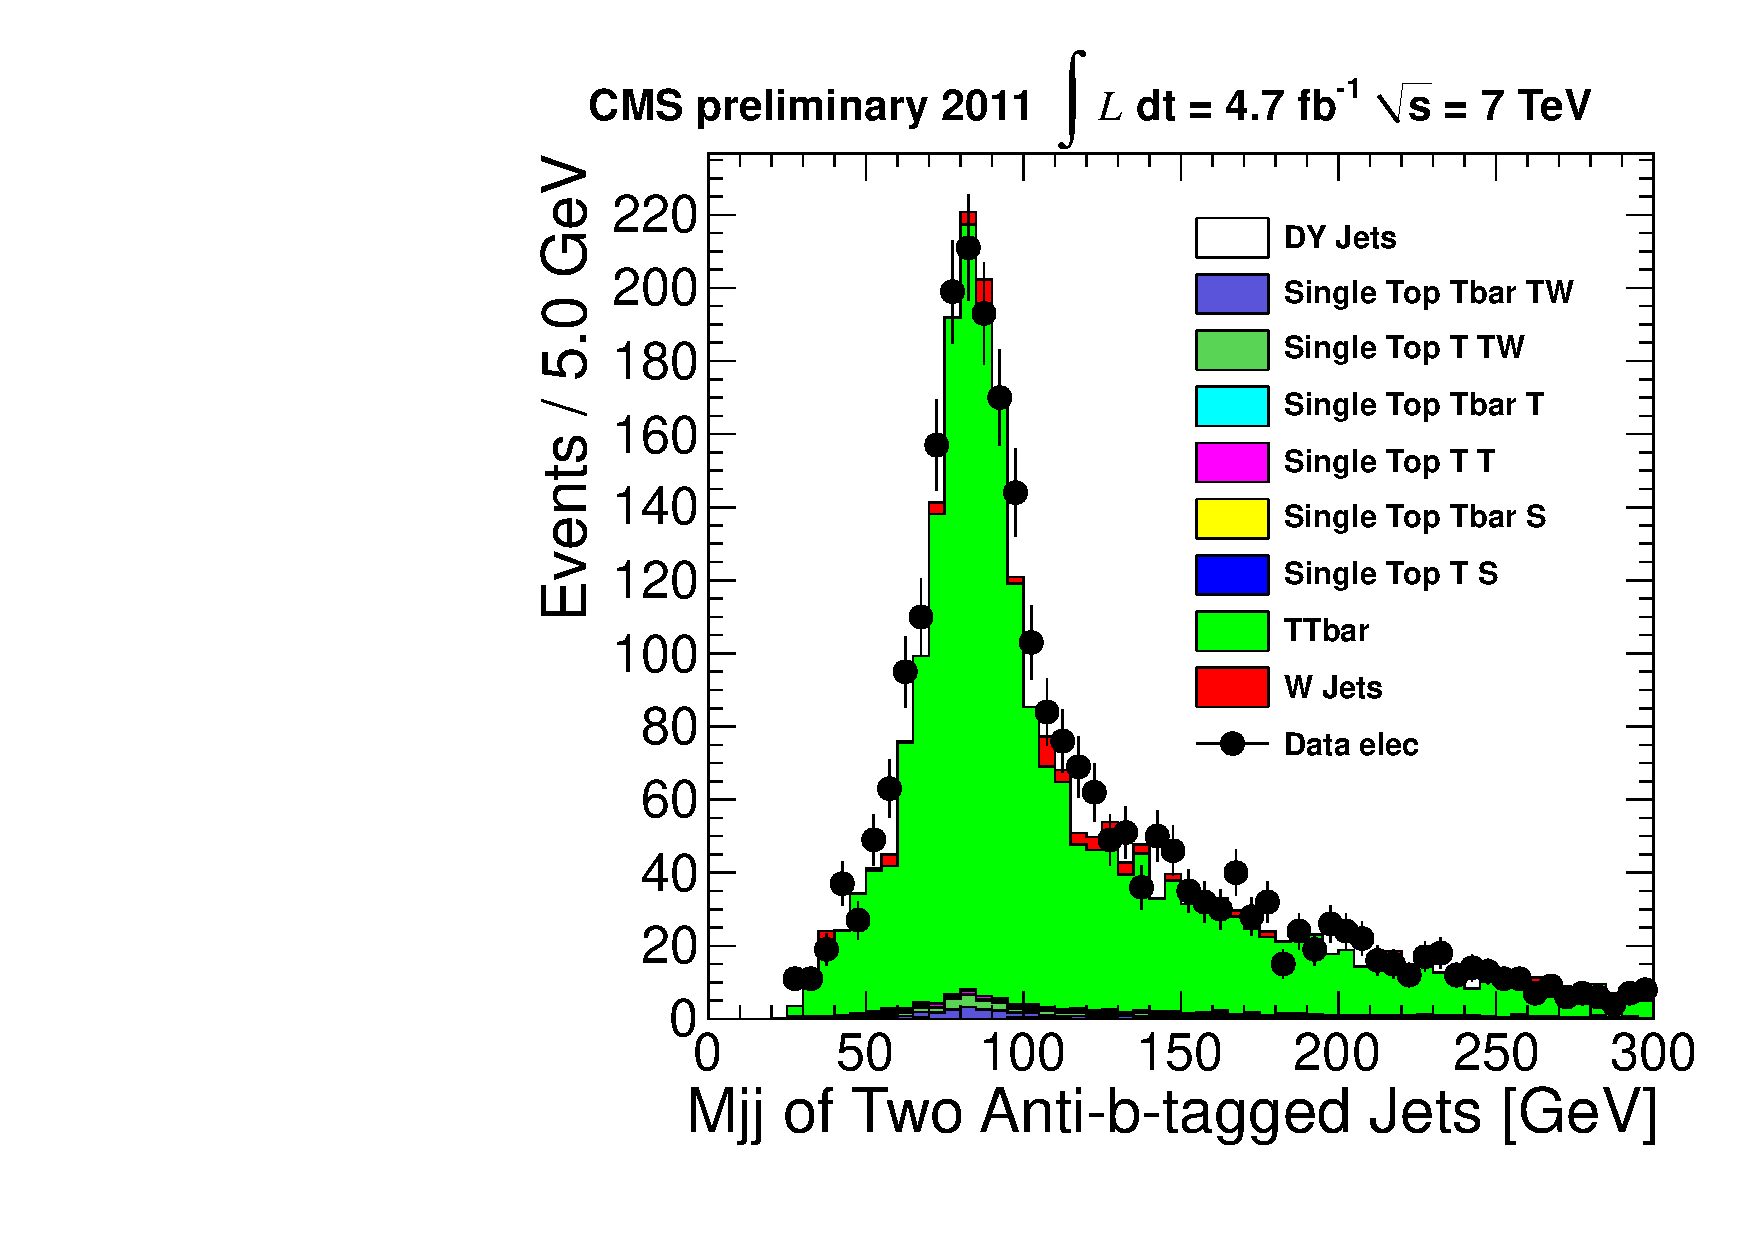
\includegraphics[width=0.75\textwidth]{figs/topwjes/top_overlap_el.pdf}
    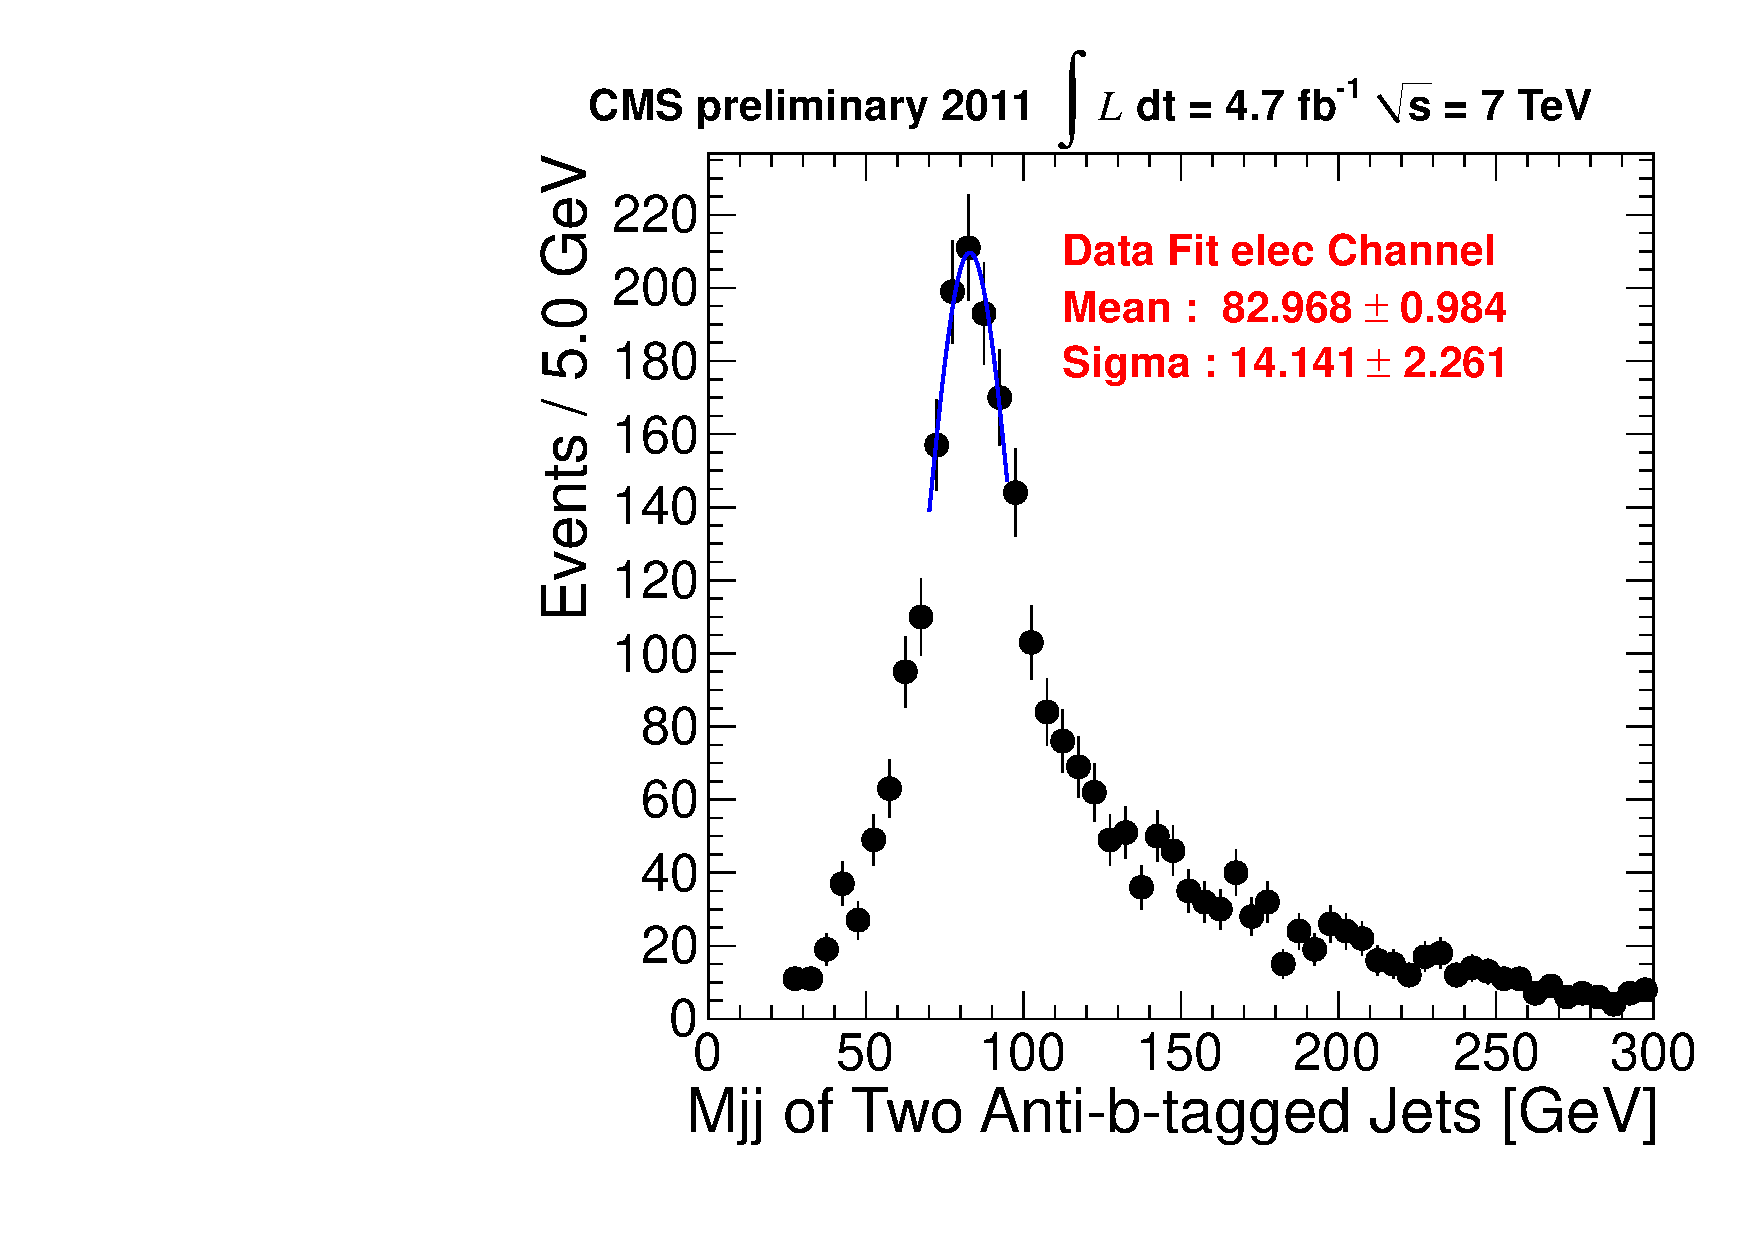
\includegraphics[width=0.49\textwidth]{figs/topwjes/top_data_fit_el.pdf}
    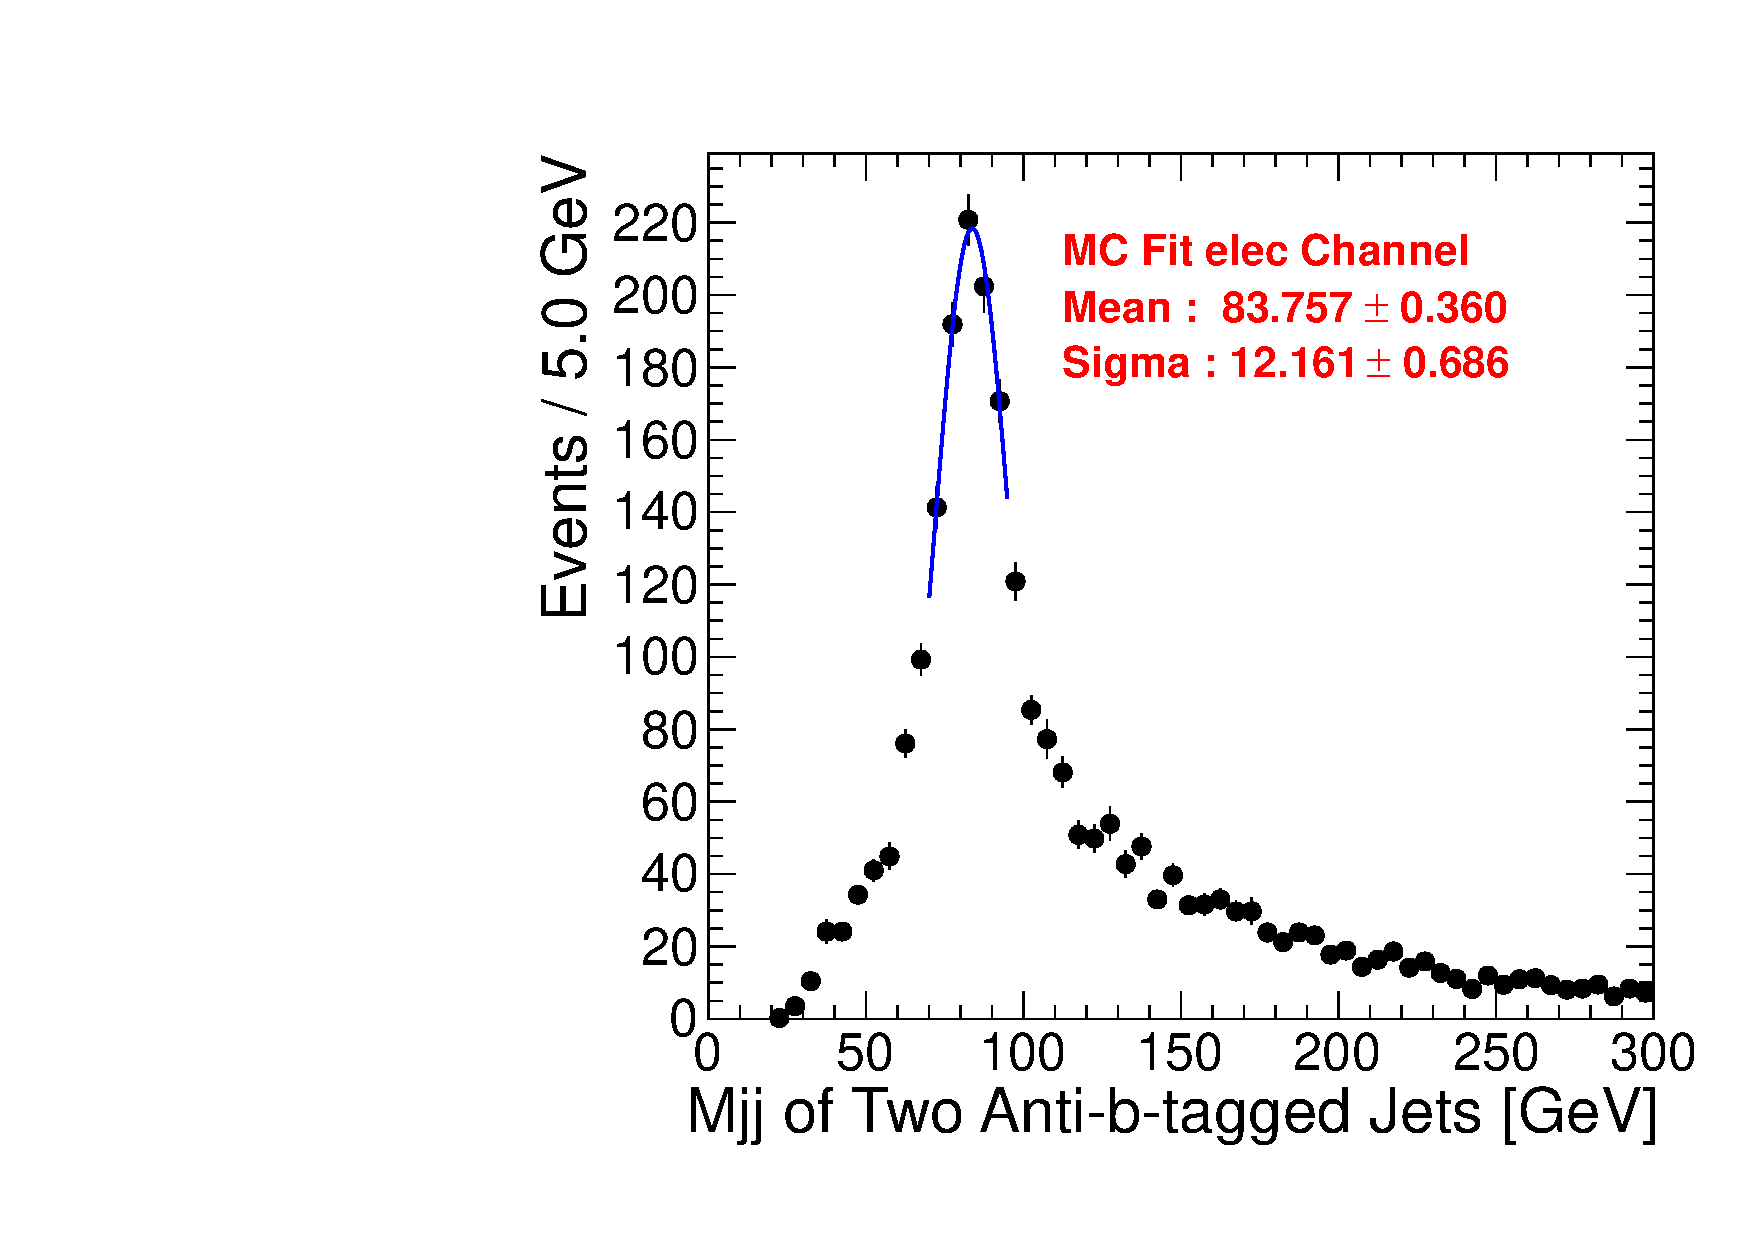
\includegraphics[width=0.49\textwidth]{figs/topwjes/top_mc_fit_el.pdf}
    \caption{The invariant mass distribution of the hadronic 
      W candidates in the electron semileptonic top sample. 
      The upper plot shows good agreement between the data and MC. 
      We fit the distribution with a Gaussian and extract the peak
      location for the data (left) and MC (right).}
    \label{fig:topw:el}}
\end{figure}
%%%%%%%%%%%%%
\begin{figure}[htb] 
  {\centering
    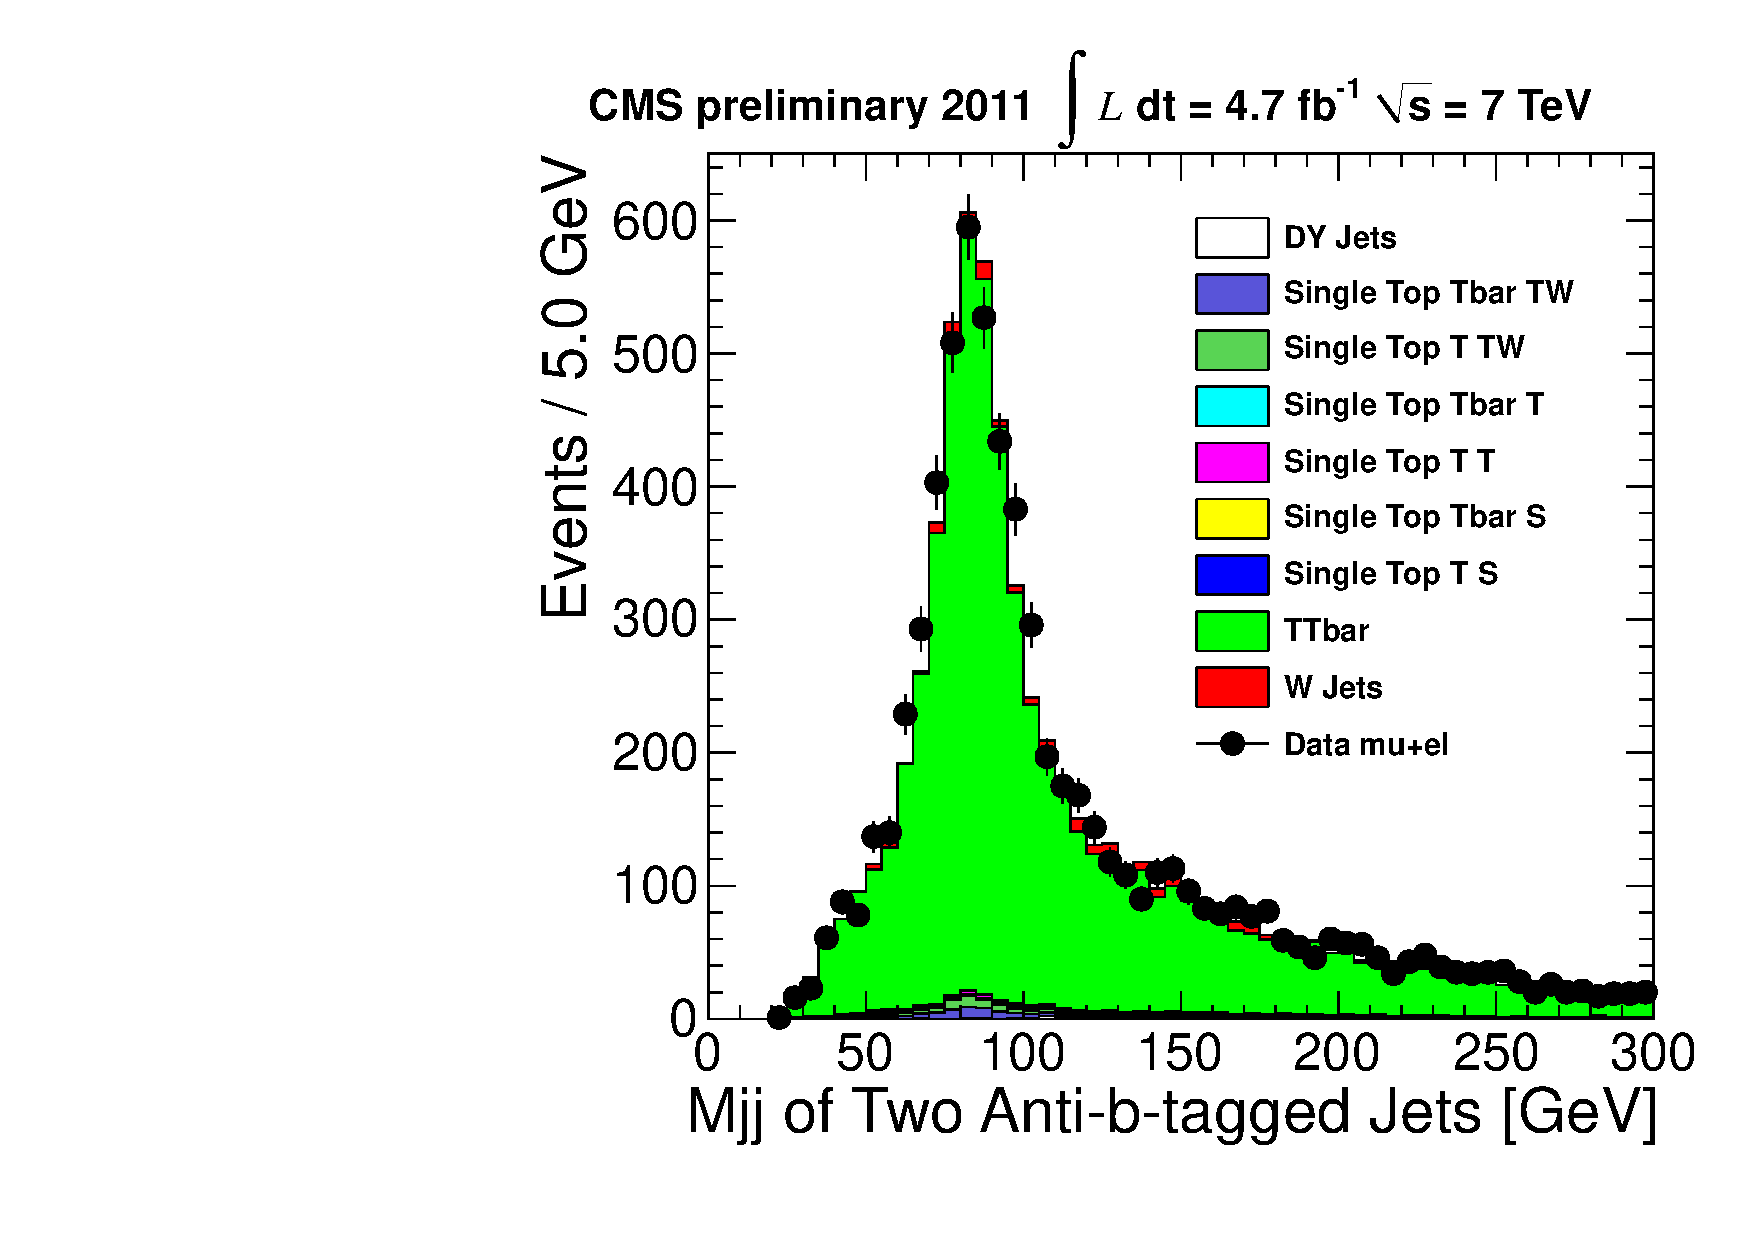
\includegraphics[width=0.75\textwidth]{figs/topwjes/top_overlap_muel.pdf}
    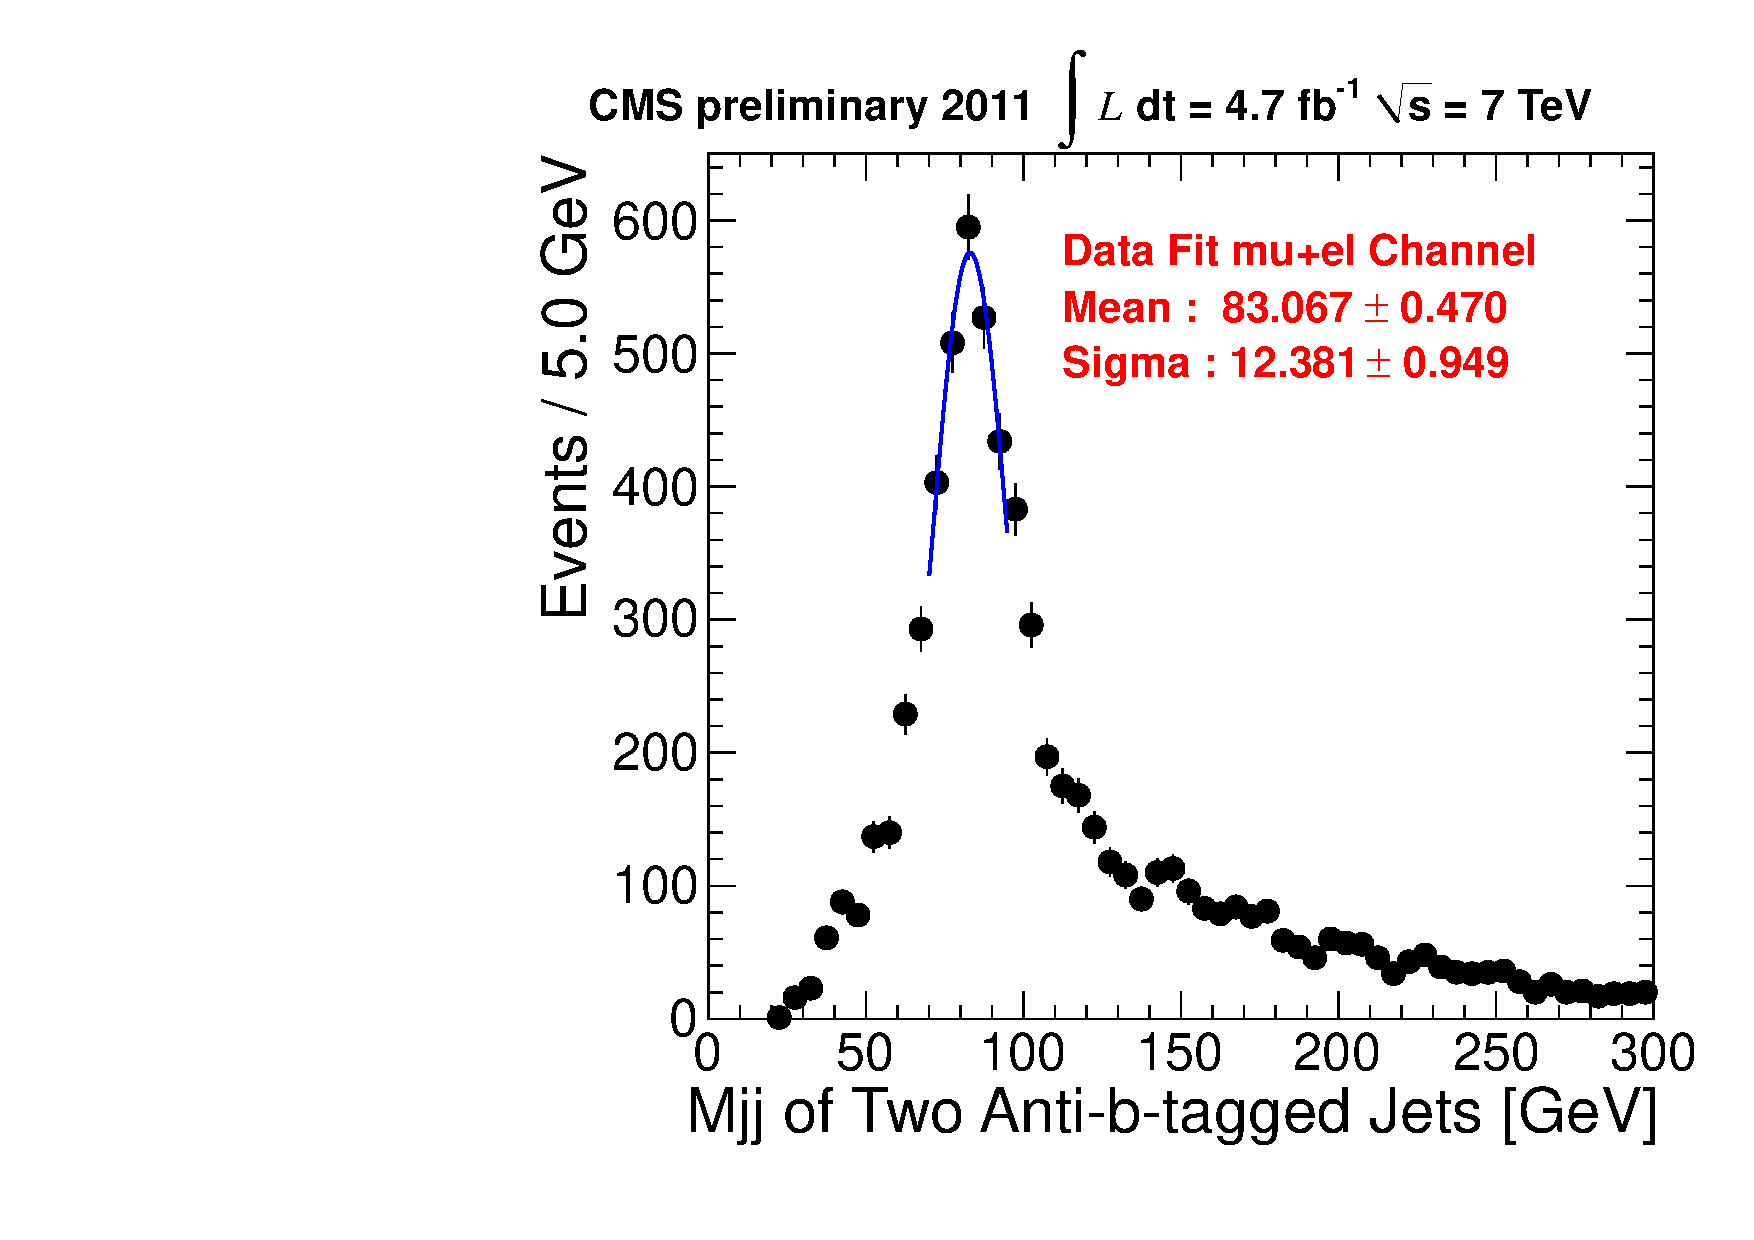
\includegraphics[width=0.49\textwidth]{figs/topwjes/top_data_fit_muel.pdf}
    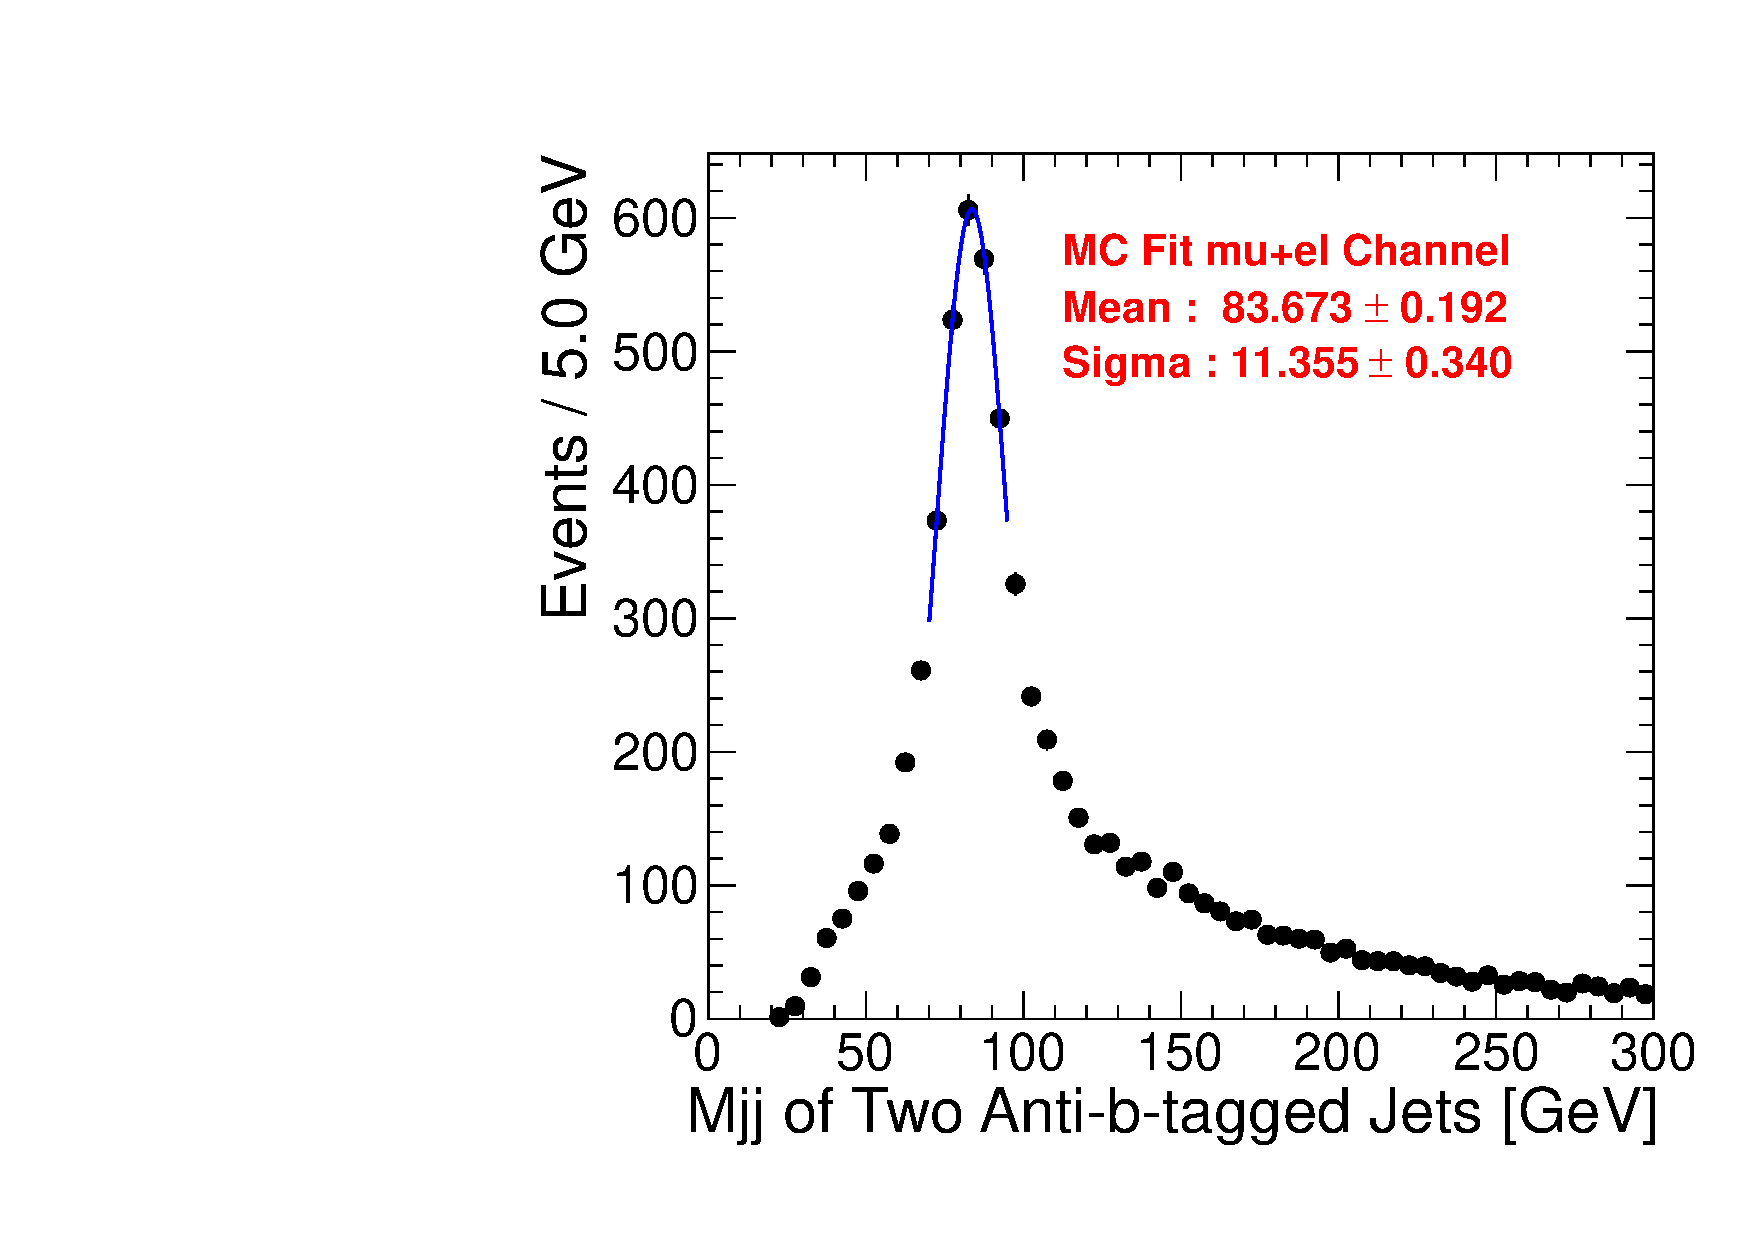
\includegraphics[width=0.49\textwidth]{figs/topwjes/top_mc_fit_muel.pdf}
    \caption{The invariant mass distribution of the hadronic 
      W candidates in the semileptonic top sample (electron and 
      muon combined). 
      The upper plot shows good agreement between the data and MC. 
      We fit the distribution with a Gaussian and extract the peak
      location for the data (left) and MC (right).}
    \label{fig:topw:muel}}
\end{figure}
%%%%%%%%%%%%%%%%%%%%%%%%%%%%%%%%%%%%%%%%%%%%%%%%%%%%%%%%%%%%%%%%%%%%%%%%%%%
%--------------------------------------------------
\subsection{Lepton selection and trigger efficiency}
\label{sec:LeptonSelectionAndTriggerEfficiency}
%%The lepton trigger and selection is common among several CMS analyses and 
%%we benefit from common studies based on tag-and-probe techniques. 
%%
Systematic uncertainties in the trigger efficiencies in Section~\ref{sec:trigger}
are of the order of 1\%. Systematic uncertainties in the lepton reconstruction
and identification efficiency scale factors are of the order of 2\%. These uncertainties
are accounted for in the final systematics that are input to the limit setter.
%--------------------------------------------------
\subsection{MET uncertainty}
MET directly affects our signal acceptance. 
The uncertainty prescription is discussed in Ref.~\cite{met}.
%https://twiki.cern.ch/twiki/bin/viewauth/CMS/MissingETUncertaintyPrescription
In addition, the MET distribution in the data is $\simeq$3\% wider 
than the MC, and placing a hard MET$>30.0$ cut creates an uncertainty. 
We estimate it by smearing the MET for each event by a Gaussian with 
a $\sigma =0.03*$MET and observing how many events pass the cut. 
Specifically, (Events Passing After Smearing)/(Events Passing Before Smearing) 
=0.998 for both muons and electrons.
%%%%%%%%%%%%%%%%%%%%%%%%%%%%
\subsection{Cross-section of nuisance backgrounds}
The uncertainty in the the cross sections of other backgrounds 
like $\ttbar$,  single top, QCD multi-jets, and Z+jets processes 
is already propagated by letting their normalization (i.e., yield) 
float in the fit within a constraint.
%%%%%%%%%%%%%%%%%%%%%%%%%%%%
\subsection{Luminosity uncertainty}
The latest recommendation for the uncertainty on LHC luminosity is 4.5$\%$~\cite{lumiPAS}.
We propagate this uncertainty to the expected yield of the New Physics 
signal while setting limits.
%%%%%%%%%%%%%%%%%%%%%%%%%%%%
